%
% $Id: ch01_overview
%
%   *******************************************************************
%   * SEE THE MAIN FILE "AllegThesis.tex" FOR MORE INFORMATION.       *
%   *******************************************************************

\chapter{Introduction}\label{ch:intro} % we can refer to chapter by the label

%   ************************************************************************
%   * In LaTeX, new paragraphs are begun by simply leaving a blank line in *
%   * the LaTeX file.                                                      *
%   *                                                                      *
%   * The \\ characters should NEVER be used to end a paragraph.           *
%   * They are used only for inserting line breaks in certain situations.  *
%   *                                                                      *
%   * "Widows" (ending paragraph lines at the top of a new page) and       *
%   * "orphans" (opening paragraph lines at the bottom of a page) should   *
%   * be eliminated; this sometimes requires re-writing some of the        *
%   * text to change the line lengths.                                     *
%   ************************************************************************

Sharing media with the public is becoming a more integral part of social interaction every day. Static images are just one of these many forms of media, and the number of daily uploads to image hosting websites is absolutely staggering. According to a recent survey by All Things Digital, as of May 2013, more than 500 million images are uploaded to image sharing websites each day, and this number is expected to double by the end of 2014 \cite{meek:500}. With figures this large, it immediately becomes apparent that multiple issues come with this trend of increased image sharing, namely, how much space does this number of images require, and is there a technology available to reduce this requirement? The simple answer is yes, there are tried and tested technologies that will reduce storage costs, but before looking into these technologies, it is important to understand what an image hosting website is and how they function.

\section{Image Hosting Services} \label{sec:imagehostingservices}
Image hosting services, or image sharing websites, are sites that allow users to upload images to the internet and share them publicly with the link they are provided. These image sharing websites mostly operate in the same fashion, but recently a new breed has emerged. As seen in Figure \ref{imageshareprocess}, both submission processes are similar, but both have inherent advantages and disadvantages.

\begin{figure}[htbp]
\centering
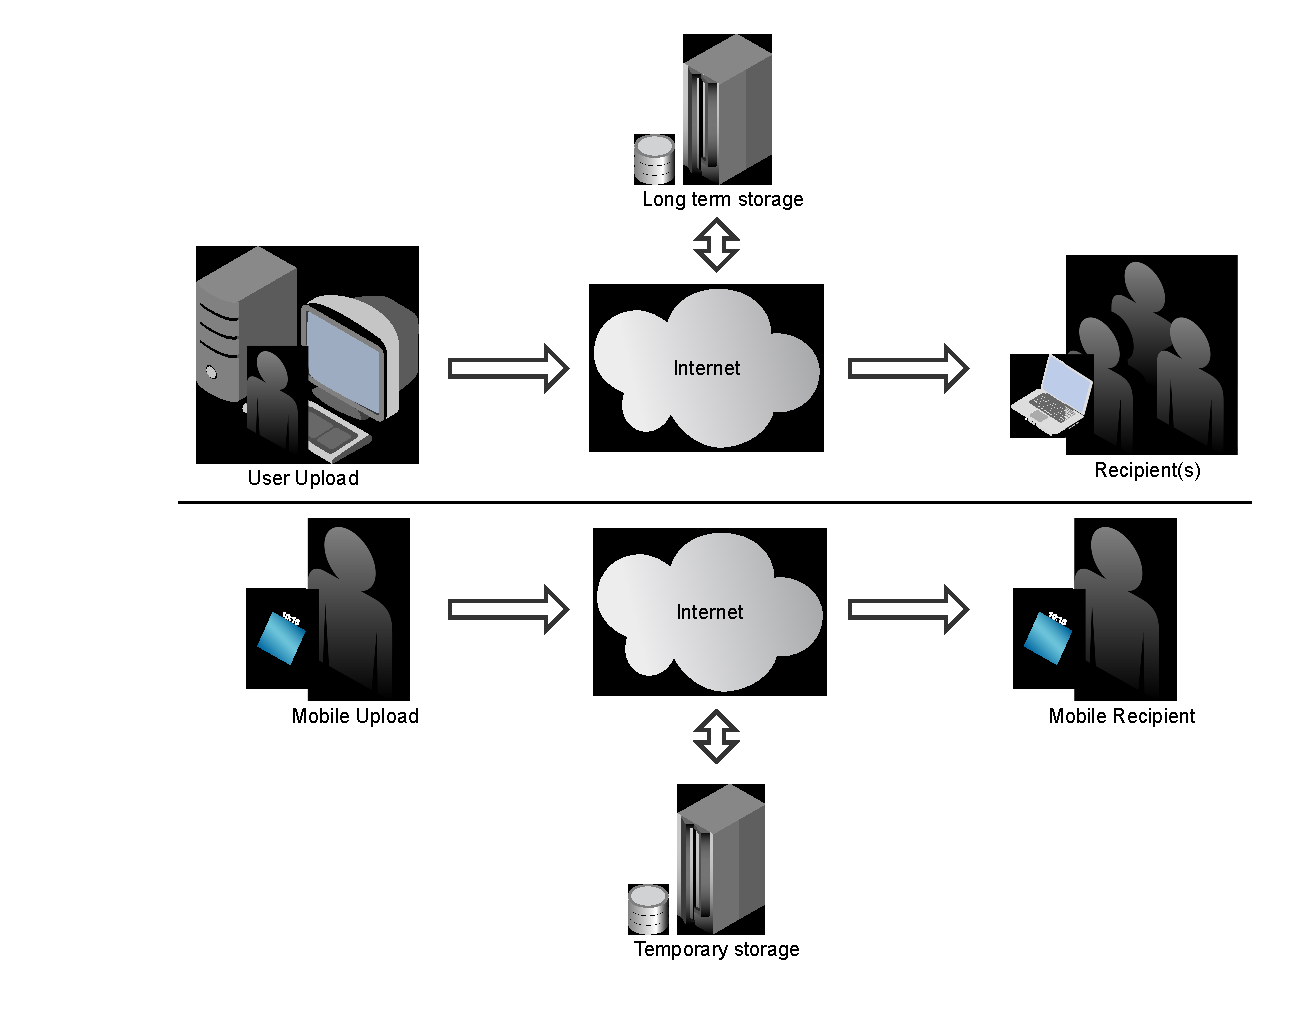
\includegraphics[width=4.5in]{imageshareprocess}
\caption{Various Image Hosting Service Structures}
\label{imageshareprocess}
\end{figure}

Looking at the first submission process variant at the top of Figure \ref{imageshareprocess}, a user would like to share an image with the public. The user can upload this image through the internet from any internet connected device, and the image will be stored on a publicly accessible server. From here, any number of people can access this shared image through an internet connected device indefinitely. Nearly all image hosting services operate on this model, some of the more popular services include but are not limited to Flickr, Imgur, Photobucket, Shutterfly, and Instagram.

The second image submission variant shown at the bottom half of Figure \ref{imageshareprocess} is currently only used by one host called Snapchat. With this system, multiple differences are immediately apparent. First, this service model will only accept images from mobile users. It can also be seen in the diagram that when a user uploads an image through the internet, it is no longer accessible long term from a server, but it is in fact only temporarily available for a specified recipient to receive. This service actually allows the uploader to set an expiration time anywhere from 1 second to 10 seconds \cite{snap:support}. After the recipient opens the image and this time period has expired, the image is deleted permanently from the server and no longer accessible to either party.

Both systems have their own inherent benefits, but they also have drawbacks. Though they reach from the infrastructure needed to support the service all the way out to the end user, this research only focuses on the infrastructure function. In order to realize the application of the proposed research, it is important to understand why such a focused application is required. For the first image hosting variant in Figure \ref{imageshareprocess}, the long term storage of image files raises concern. By storing files for an extended period of time, it is a guarantee that duplicate data will eventually make its way to the storage servers. Determining duplicates and preventing their addition can save not only a considerable amount of space as the amount of redundant data increases, but it can also save a large amount of money when discussing the cost per gigabyte of data storage. This research will not target the application of the temporary system seen at the bottom of the figure as the amount of stored data is minimal due to the rapid turnover of data being housed.

\section{Data Management Technologies} \label{sec:datadeduptech}
The image hosting services outlined in section \ref{sec:imagehostingservices} utilize numerous technologies to help lessen the load of the files they must store. Though official word and articles discussing the technologies these companies implement are nonexistent, after examining the services several different technologies became immediately apparent. The most prominent method of space reduction is the reduction in size of uploaded images. By reducing the quality of the image by a small percent, these websites are able to significantly reduce the amount of space needed to store the uploaded images. The next most common method of space reduction used is the expiration of uploads. After locating the earliest available images across the websites it was determined that the file expiration can possibly work in one of two ways. The implementation either functions as a countdown from the date of upload or in the other case the countdown begins after the last date the file was accessed. Each time the file is accessed, the timer will reset. Finally, some of these sites also limit the size of the uploaded files and the number of uploads per user. In order to remove these restrictions, many sites also offer paid services which assist with the cost of upkeep. 

\section{Motivation} \label{sec:motivation}
Summarizing the information presented thus far, image hosting websites clearly require complex infrastructures, not only to allow the sharing of files but to manage the large numbers of submissions. Although the numerous technologies used to lessen the space requirements of the submissions work well, it should be possible to further improve on the system by reducing the number of duplicate submissions. According to a recent survey by All Things Digital, more than 500 million images are uploaded to long-term image sharing websites, and this number is expected to double by the end of 2014 \cite{meek:500}. In addition, a study published by NTP Software found that nearly 20\% of stored data is duplicate \cite{ntps:staledata}. These numbers are staggering, especially when there is a possibility of reducing an additional 100 million images.

To bring the possible savings into light a rough calculation based on the 2013 average of \$.05 per gigabyte and an assumed image size of 1MB will show that by removing the duplicates a significant amount of money could be saved. More specifically, approximately \$18 million can be saved annually at the current sharing levels. By allowing unregulated user submitted data, it quickly becomes apparent that data redundancy reduction can save a significant amount of storage space and money.

\section{Goals of the Project}\label{sec:goals}
The purpose of this project is to develop and test a system capable of identifying and reducing the number of duplicate image submissions on an image sharing website. In order to fulfill this goal, an image sharing website will be developed that is capable of accepting images as uploads and providing a link to the user for public access of the image. To develop a functional website it must be able to perform several functions. This website should accept an image file through an online submission form. At this point, it will process the image and match it against the collection of images currently stored on the server. This process will be completed using a series of algorithms and checks outlined in in section \ref{ch:method}. The website will also be developed using PHP, the PHP GD image library, and HTML5 to ensure minimal chance of conflicts between scripts and languages. Using this website, the proposed duplicate image detection tool will be implemented using both original and existing code from other resources and tested thoroughly to assess the effectiveness of using this method of duplicate reduction.

\section{Thesis Outline}\label{sec:outline}
The remainder of this thesis will discuss the work in further detail in addition to existing information relating to the topic. The first topic being discussed is Chapter \ref{ch:relatedwork}, which covers related works and existing research that has been completed on the topic of image matching and comparison. Chapter \ref{ch:method} will cover the project details pertaining to the website and supporting infrastructure it will operate on. This will include a brief discussion of the hardware and configuration of the web server in addition to the website design and implementation of the duplicate image detection tool that will be integrated and tested. Chapter \ref{ch:reseval} will then discuss the collected results and the accompanying evaluation of the collected data. This evaluation will include the performance costs of implementing this system over a passive one, which only acts to prevent a specific file from ever being submitted to the server. The evaluation will also include the results of the image de-duplication and a determination of whether such a system is a feasible method of reducing storage requirements. An additional section outlining threats to validity will also be included in this chapter. Finally, Chapter \ref{ch:conclusion} will summarize the research and conclusions completed throughout this Senior Comprehensive Project and include possible areas of future work.